\documentclass[12pt]{report}
\usepackage[utf8]{inputenc}
\usepackage[russian]{babel}
%\usepackage[14pt]{extsizes}
\usepackage{listings}

% Для листинга кода:
\lstset{ %
language=python,                 % выбор языка для подсветки 
basicstyle=\small\sffamily, % размер и начертание шрифта для подсветки кода
numbers=left,               % где поставить нумерацию строк (слева\справа)
numberstyle=\tiny,           % размер шрифта для номеров строк
stepnumber=1,                   % размер шага между двумя номерами строк
numbersep=5pt,                % как далеко отстоят номера строк от подсвечиваемого кода
showspaces=false,            % показывать или нет пробелы специальными отступами
showstringspaces=false,      % показывать или нет пробелы в строках
showtabs=false,             % показывать или нет табуляцию в строках            
tabsize=2,                 % размер табуляции по умолчанию равен 2 пробелам
captionpos=t,              % позиция заголовка вверху [t] или внизу [b] 
breaklines=true,           % автоматически переносить строки (да\нет)
breakatwhitespace=false, % переносить строки только если есть пробел
escapeinside={\#*}{*)}   % если нужно добавить комментарии в коде
}

% Для измененных титулов глав:
\usepackage{titlesec, blindtext, color} % подключаем нужные пакеты
\definecolor{gray75}{gray}{0.75} % определяем цвет
\newcommand{\hsp}{\hspace{20pt}} % длина линии в 20pt
% titleformat определяет стиль
\titleformat{\chapter}[hang]{\Huge\bfseries}{\thechapter\hsp\textcolor{gray75}{|}\hsp}{0pt}{\Huge\bfseries}


% plot
\usepackage{pgfplots}
\usepackage{filecontents}
\usepackage{amsmath}
\usepackage{tikz,pgfplots}
\usetikzlibrary{datavisualization}
\usetikzlibrary{datavisualization.formats.functions}
\begin{filecontents}{stdgood.dat}
100  0.5494
200 4.15013
300 14.72735
400 34.76485
\end{filecontents}
\begin{filecontents}{winogradgood.dat}
100  0.69569
200 4.66497
300 16.41758
400 40.25307
\end{filecontents}
\begin{filecontents}{impwinogradgood.dat}
100  0.56495
200 4.54574
300 14.99365
400 36.63559
\end{filecontents}

\begin{filecontents}{stdmal.dat}
101  0.59867
201 4.61544
301 14.79835
401 35.3947
501 72.95269
\end{filecontents}
\begin{filecontents}{winogradmal.dat}
101  0.68139
201 5.01175
301 16.28355
401 40.06329
501 83.25553
\end{filecontents}
\begin{filecontents}{impwinogradmal.dat}
100  0.61839
200 4.46456
300 14.74381
400 37.95568
500 72.76217
\end{filecontents}

\usepackage{graphicx}
\graphicspath{{src/}}
\DeclareGraphicsExtensions{.pdf,.png,.jpg}

\begin{document}
%\def\chaptername{} % убирает "Глава"
\begin{titlepage}
	\centering
	{\scshape\LARGE МГТУ им. Баумана \par}
	\vspace{3cm}
	{\scshape\Large Рубежный контроль №1\par}
	\vspace{0.5cm}	
	{\scshape\Large По курсу: "Анализ алгоритмов"\par}
	\vspace{1.5cm}
	{\huge\bfseries Эффективная реализация алгоритма винограда\par}
	\vspace{2cm}
	\Large Работу выполнил: Лумбунов Дмитрий, ИУ7-54\par
	\vspace{0.5cm}
	\Large Преподаватели:  Волкова Л.Л., Строганов Ю.В.\par

	\vfill
	\large \textit {Москва, 2019} \par
\end{titlepage}

\tableofcontents

\newpage
\chapter*{Введение}
\addcontentsline{toc}{chapter}{Введение}

Цель работы: изучение методов оптимизации алгоритмов. В данной лабораторной работе рассматривается стандартный алгоритм умножения матриц и модифицированный алгоритм Винограда.  Также требуется сравнить временные характеристики данных алгоритмов.

В ходе работы предстоит:
\begin{itemize}
	\item изучить алгоритмы умножения матриц: стандартный и алгоритм Винограда; 
	\item оптимизировать алгоритм Винограда; 
	\item дать теоретическую оценку базового алгоритма умножения матриц и улучшенного алгоритма Винограда;
	\item реализовать два алгоритма умножения матриц на одном из языков программирования;  
	\item сравнить временные характеристики алгоритмов умножения матриц.
\end{itemize}

\chapter{Аналитическая часть}
Матрицей A размера $[m*n]$ называется прямоугольная таблица
чисел, функций или алгебраических выражений, содержащая m строк и n столбцов. Числа m и n определяют размер матрицы.\cite{Beloysov} Если число столбцов в первой матрице совпадает с числом строк во второй, то эти две матрицы можно перемножить. У произведения будет столько же строк, сколько в первой матрице, и столько же столбцов, сколько во второй.

Пусть даны две прямоугольные матрицы А и В размеров $[m * n]$ и $[n * k]$ соответственно.  
В результате произведение матриц A и B получим матрицу C размера $[m *  k]$.


$c_{i,j} = \sum\limits_{r=1}^n a_{i,r}\cdot b_{r,j}$ называется произведением матриц A и B \cite{Beloysov}.


\section{Алгоритм Винограда}
Подход Алгоритма Винограда является иллюстрацией общей методологии, начатой в 1979-х годах на основе
билинейных и трилинейных форм, благодаря которым большинство усовершенствований для умножения матриц были получены \cite{Gall2012}.

Рассмотрим два вектора $V = (v1, v2, v3, v4)$ и $W = (w1, w2, w3, w4)$.  

Их скалярное произведение равно (\ref{formula}) 

\begin{equation} \label{formula}
V \cdot W=v_1 \cdot w_1 + v_2 \cdot w_2 + v_3 \cdot w_3 + v_4 \cdot w_4
\end{equation}

Равенство (\ref{formula}) можно переписать в виде (\ref{formula2}) 
\begin{equation} \label{formula2}
V \cdot W=(v_1 + w_2) \cdot (v_2 + w_1) + (v_3 + w_4) \cdot (v_4 + w_3) - v_1 \cdot v_2 - v_3 \cdot v_4 - w_1 \cdot w_2 - w_3 \cdot w_4
\end{equation}

Менее очевидно, что выражение в правой части последнего равенства допускает предварительную обработку: его части можно вычислить заранее и запомнить для каждой строки первой матрицы и для каждого столбца второй. 
Это означает, что над предварительно обработанными элементами нам придется выполнять лишь первые два умножения и последующие пять сложений, а также дополнительно два сложения. 

\section{Вывод}
Были рассмотрены алгоритмы классического умножения матриц и алгоритм Винограда, основное отличие которых — наличие предварительной обработки, а также количество операций умножения.

\chapter{Конструкторская часть}
\textbf{Требования к вводу:}
На вход подаются две матрицы
\newline
\textbf{Требования к программе:}
\begin{itemize}
	\item корректное умножение двух матриц;
	\item при матрицах неправильных размеров программа не должна аварийно завершаться.
\end{itemize}

\section{Схемы алгоритмов}
В данной части будут рассмотрены схемы алгоритмов.

\begin{figure}[!htbp]
	\centering
	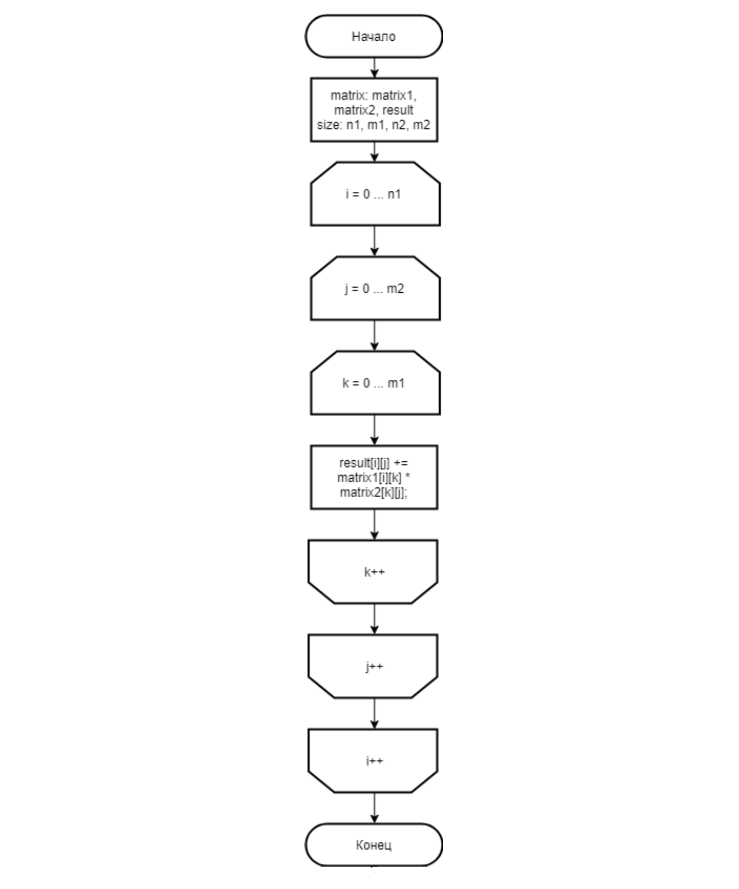
\includegraphics[scale=1]{m_std.png}
	\caption{Схема классического алгоритма умножения матриц}
	\label{fig:mpr}
\end{figure}

\begin{figure}[!htbp]
	\centering
	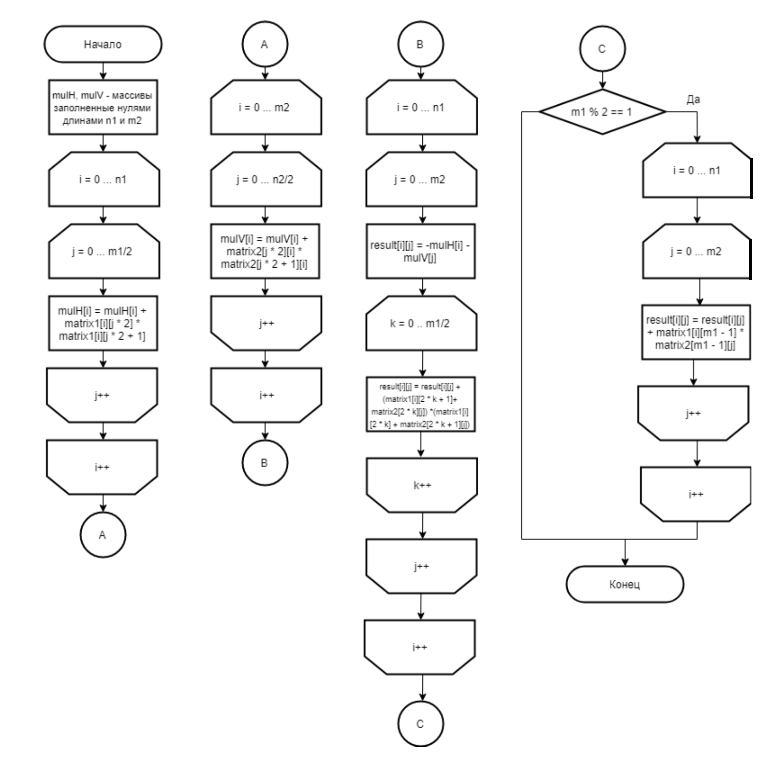
\includegraphics[scale=1]{m_winograd.png}
	\caption{Схема алгоритма Винограда}
	\label{fig:mpr}
\end{figure}


\begin{figure}[!htbp]
	\centering
	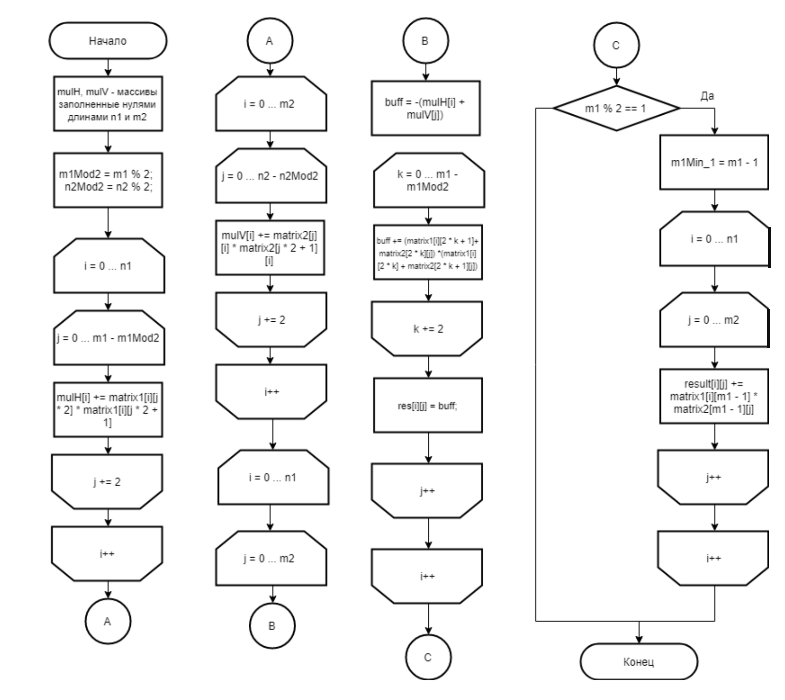
\includegraphics[scale=1]{imp_winograd}
	\caption{Схема оптимизированного алгоритма Винограда}
	\label{fig:mpr}
\end{figure}

\newpage
\section{Трудоемкость алгоритмов}
Введем модель трудоемкости для оценки алгоритмов: 
\begin{itemize}
	\item базовые операции стоимостью 1 — +, -, *, /, =, ==, <=, >=, !=, +=, [], получение полей класса
	\item оценка трудоемкости цикла: Fц = init +  N*(a + Fтела + post) + a, где a - условие цикла, init - предусловие цикла, post - постусловие цикла
	\item стоимость условного перехода применим за 0, стоимость вычисления условия остаётся
\end{itemize}

Оценим трудоемкость алгоритмов по коду программы.

\subsection{Классический алгоритм}
Рассмотрим трудоемкость классического алгоритма:  

Инициализация матрицы результата: $1 + 1 + n_1(1 + 2 + 1) + 1 = 4n_1 + 3$

Подсчет:\\
$1 + n_1(1 + (1 + m_2(1 + (1 + m_1(1 + (8) + 1) + 1) + 1) + 1) + 1) + 1 = 
n_1(m_2(10m_1 + 4) + 4) + 4) + 2 = 10n_1m_2m_1+ 4n_1m_2 + 4n_1 +2
$

\subsection{Оптимизированный алгоритм Винограда}

Аналогично Рассмотрим трудоемкость оптимизированого алгоритма Винограда:\\

Первый цикл: $\frac{11}{2}n_1m_1 + 4n_1 + 2$ 

Второй цикл: $\frac{11}{2}m_2n_2+ 4m_2 + 2$

Третий цикл: $\frac{17}{2}n_1m_2m_1 + 9n_1m_2 + 4n_1 + 2$

Условный переход: $\begin{bmatrix}
1    &&, \text{невыполнение условия}\\
10n_1m_2 + 4n_1 + 2 &&, \text{выполнение условия}\\
\end{bmatrix} $ \\

Итого: $\frac{17}{2}n_1m_2m_1 + \frac{11}{2}n_1m_1 + \frac{11}{2}m_2n_2 + 9n_1m_2 + 8n_1 + 4m_2 + 6 + \\
\begin{bmatrix}
1    &&, \text{невыполнение условия}\\
10n_1m_2 + 4n_1 + 2 &&, \text{выполнение условия}\\
\end{bmatrix} $ \\

\section{Вывод}
В данном разделе были рассмотрены схемы алгоритмов умножения матриц, введена модель оценки трудоемкости алгоритма, были расчитаны трудоемкости алгоритмов в соответсвии с этой моделью.

\chapter{Технологическая часть}
\section{Выбор ЯП}
Я выбрал в качестве Python языком программирования, потому как он достаточно удобен и гибок.

Время работы алгоритмов было замерено с помощью функции time() из библиотеки time.

\section{Описание структуры ПО}
\begin{figure}[h]
	\centering
	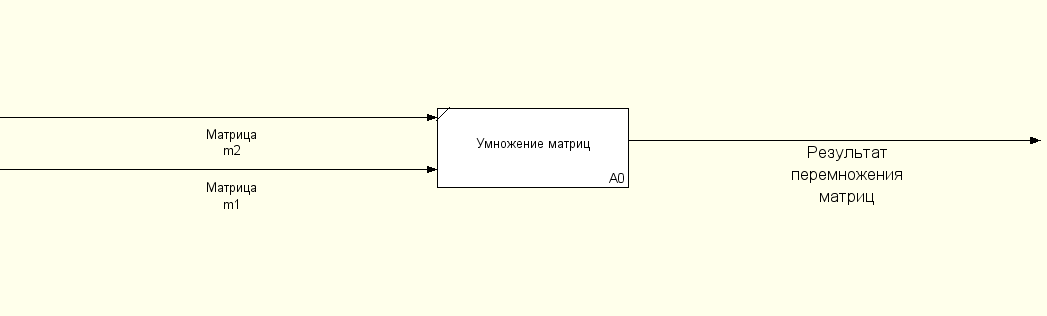
\includegraphics[width=1.25\linewidth]{lab02ram}
	\caption{Функциональная схема умножения матриц (IDEF0 диаграмма 1 уровня)}
	\label{fig:mpr}
\end{figure}

\section{Сведения о модулях программы}
Программа состоит из:
\begin{itemize}
	\item lab02.py - главный файл программы, в котором располагается точка входа в программу и функция замера времени.
\end{itemize}

\section{Листинг кода алгоритмов}

\begin{lstlisting}[label=CodeStand,caption= Стандартный алгоритм умножения матриц]
def std(mtr1, mtr2):
	if len(mtr2) != len(mtr1[0]):
		print("Wrong size of matrix")
		return

	row1 = len(mtr1); col1 = len(mtr1[0])
	col2 =  len(mtr2[0])

	res = [[0 for i in range(col2)] for j in range(row1)]
	for i in range(row1):
		for j in range(col1):
			for k in range(col2):
				res[i][k] += mtr1[i][j] * mtr2[j][k]
	return res
\end{lstlisting}

\begin{lstlisting}[label=winograd_opt,caption=Оптимизированный алгорит Винограда]
def imp_winograd(mtr1, mtr2):
	row1 = len(mtr1)
	row2 = len(mtr2)
	col2 = len(mtr2[0])

	if row2 != len(mtr1[0]):
		print("Different dimension of the matrics")
		return

	d = row2 // 2

	row_factor = [0 for i in range(row1)]
	col_factor = [0 for i in range(col2)]

	for i in range(row1):
		row_factor[i] = sum(mtr1[i][2 * j] * mtr1[i][2 * j + 1] for j in range(d))

	for i in range(col2):
		col_factor[i] = sum(mtr2[2 * j][i] * mtr2[2 * j + 1][i] for j in range(d))

	answer = [[0 for i in range(col2)] for j in range(row1)]
	for i in range(row1):
		for j in range(col2):
			answer[i][j] = sum((mtr1[i][2 * k] + mtr2[2 * k + 1][j]) * (mtr1[i][2 * k + 1] + mtr2[2 * k][j]) for k in range(d))\
			- row_factor[i] - col_factor[j]

	if row2 % 2:
		for i in range(row1):
			answer[i][j] = sum(mtr1[i][row2 - 1] * mtr2[row2 - 1][j] for j in range(col2))

	return answer
\end{lstlisting}

\subsection{Оптимизация алгоритма Винограда}
В рамках данной работы было предложено 3 оптимизации:
\begin{enumerate}
	\item Избавление от деления в условии цикла;
	\newpage
	\begin{lstlisting}[label=some-code,caption=Оптимизации алгоритма Винограда №1 и №2]
    for i in range(row1):
		row_factor[i] = sum(mtr1[i][2 * j] * mtr1[i][2 * j + 1] for j in range(d))

	for i in range(col2):
		col_factor[i] = sum(mtr2[2 * j][i] * mtr2[2 * j + 1][i] for j in range(d))

	\end{lstlisting}
	
	\item Накопление результата в буфер, чтобы не обращаться каждый раз к одной и той же ячейке памяти.
	\begin{lstlisting}[label=some-code,caption=Оптимизации алгоритма Винограда №3]
    for i in range(row1):
		for j in range(col2):
			answer[i][j] = sum((mtr1[i][2 * k] + mtr2[2 * k + 1][j]) * (mtr1[i][2 * k + 1] + mtr2[2 * k][j]) for k in range(d))\
			- row_factor[i] - col_factor[j]
	\end{lstlisting}
\end{enumerate}

\section{Вывод}
В данном разделе была рассмотрена структура ПО и листинги кода программы.

\chapter{Исследовательская часть}
Был проведен замер времени работы каждой из сортировок.
\section{Примеры работы}
\begin{figure}[h]
	\center{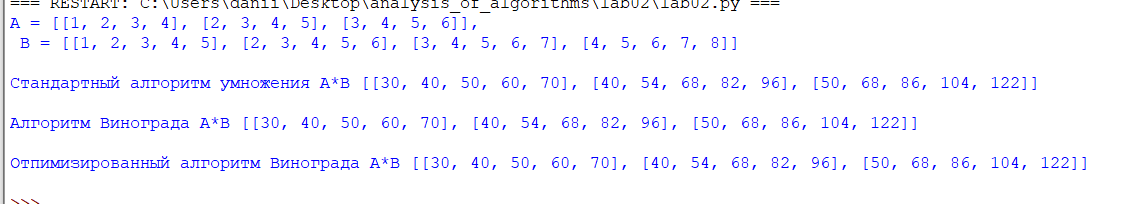
\includegraphics[scale=0.9]{example.png}} 
	\caption{Пример работы программы}
	\label{ris:example}
\end{figure}


\section{Постановка эксперемента}
Проведем сравнение для каждого из алгоритмов. Для замера времени будем использовать функцию time.
\newpage
\subsection{Лучший случай}
Квадратные матрицы с четным размером матриц size * size
\begin{center}
	\begin{tabular}{|c c c c|} 
 	\hline
	size & sdt & winograd & improwed winograd \\ [0.5ex] 
 	\hline\hline
 	100 & 0.5494 & 0.69569 & 0.56495 \\
 	\hline
 	200 & 4.15013 & 4.66497 & 4.54574\\
 	\hline
	300 & 14.72735 & 16.41758 & 14.99365 \\
	\hline
	400 & 34.76485 & 40.25307 & 36.63559 \\
	\hline
	500 & 0.08998 & 0.10028 & 0.16667\\
	\hline
	\end{tabular}
\end{center}


\begin{figure}
\begin{tikzpicture}
\begin{axis}[
    	axis lines = left,
    	xlabel = $size$,
    	ylabel = {$time$},
	legend pos=north west,
	ymajorgrids=true
]
\addplot[color=red] table[x index=0, y index=1] {stdgood.dat}; 
\addplot[color=green] table[x index=0, y index=1] {winogradgood.dat};
\addplot[color=blue, mark=square] table[x index=0, y index=1] {impwinogradgood.dat};

\addlegendentry{std}
\addlegendentry{winograd}
\addlegendentry{impwinograd}
\end{axis}
\end{tikzpicture}
\caption{Сравнение алгоритмов на матрицах четных размеров} \label{plot:even}
\end{figure}
\par

\subsection{Худший случай}
Квадратные матрицы с нечетным размером матриц size * size
\begin{center}
	\begin{tabular}{|c c c c|} 
 	\hline
	size & sdt & winograd & improwed winograd \\ [0.5ex] 
 	\hline\hline
 	101 & 0.59867 & 0.68139 & 0.61839 \\
 	\hline
 	201 & 4.61544 & 5.01175 & 4.46456\\
 	\hline
	301 & 14.79835 & 16.28355 & 14.74381 \\
	\hline
	401 & 35.3947 & 40.06329 & 37.95568\\
	\hline
	501 & 72.95269 & 83.25553 & 72.76217\\
	\hline
	\end{tabular}
\end{center}






\newpage
\subsection{Заключение эксперементальной части}
Были протестированы алгоритмы умножения матриц на массивах размерами 100х100 … 500х500 с шагом 100х100.

В результате тестирования было получено, что лучшее время умножения показывает улучшенный алгоритм винограда при больших размерах матриц. При малых размерах матриц, рассмотренных в работе, целесообразнее использовать стандартный алгоритм умножения матриц.

\chapter*{Заключение}
\addcontentsline{toc}{chapter}{Заключение}

В ходе выполнения данной работы были проанализированы стандартный алгоритм умножения матриц и оптимизированный алгоритм Винограда.

Оптимизации, примененные к алгоритму Винограда, ни при каких условиях не замедляют вычисления. Оптимизированный алгоритм Винограда на всех данных показал лучшие результаты, чем стандартный алгоритм Винограда, но всё же хуже по сравнению со стандартным алгоритмом умножения матриц.

В результате тестирования было получено, что лучшее время умножения показывает улучшенный алгоритм винограда при больших размерах матриц. При малых размерах матриц целесообразнее использовать стандартный алгоритм умножения матриц.

Алгоритм Винограда выигрывает у стандартного засчет возможности предварительной обработки данных, однако сами же вычисления в алгоритме Винограда содержат большее количество операций, что делает его неэффективным в ситуациях, когда предварительная обработка данных не играет роли, т.е. при малых размерах матриц.

На практике алгоритм Копперсмита—Винограда не используется, так как он имеет очень большую константу пропорциональности и начинает выигрывать в быстродействии у других известных алгоритмов только для матриц, размер которых превышает память современных компьютеров.




\addcontentsline{toc}{chapter}{Список литературы}
\begin{thebibliography}{3}
	\bibitem{Beloysov}
	И. В. Белоусов(2006), Матрицы и определители, учебное пособие по линейной алгебре, с. 1 - 16
	\bibitem{Gall2012}
	Le Gall, F. (2012), "Faster algorithms for rectangular matrix multiplication", Proceedings of the 53rd Annual IEEE Symposium on Foundations of Computer Science (FOCS 2012), pp. 514–523
	%https://arxiv.org/pdf/1204.1111.pdf
	\bibitem{Microsoft}
	Руководство по языку C\#[Электронный ресурс], - режим доступа: https://docs.microsoft.com/ru-ru/dotnet/csharp/
\end{thebibliography}

\end{document}
